%%%%%%%%%%%%%%%%%%%%%%%%%%%
% Author : Paul Gaborit (2009)
% under Creative Commons attribution license.
% Title : Pascal's triangle and Sierpinski triangle
% Note : 17 lines maximum
\documentclass[landscape]{article}
\usepackage[landscape,margin=1cm]{geometry}
\pagestyle{empty}
\usepackage[T1]{fontenc}
\usepackage{lmodern}

\usepackage{tikz}
\usetikzlibrary{positioning,shadows,backgrounds}
\begin{document}
\centering

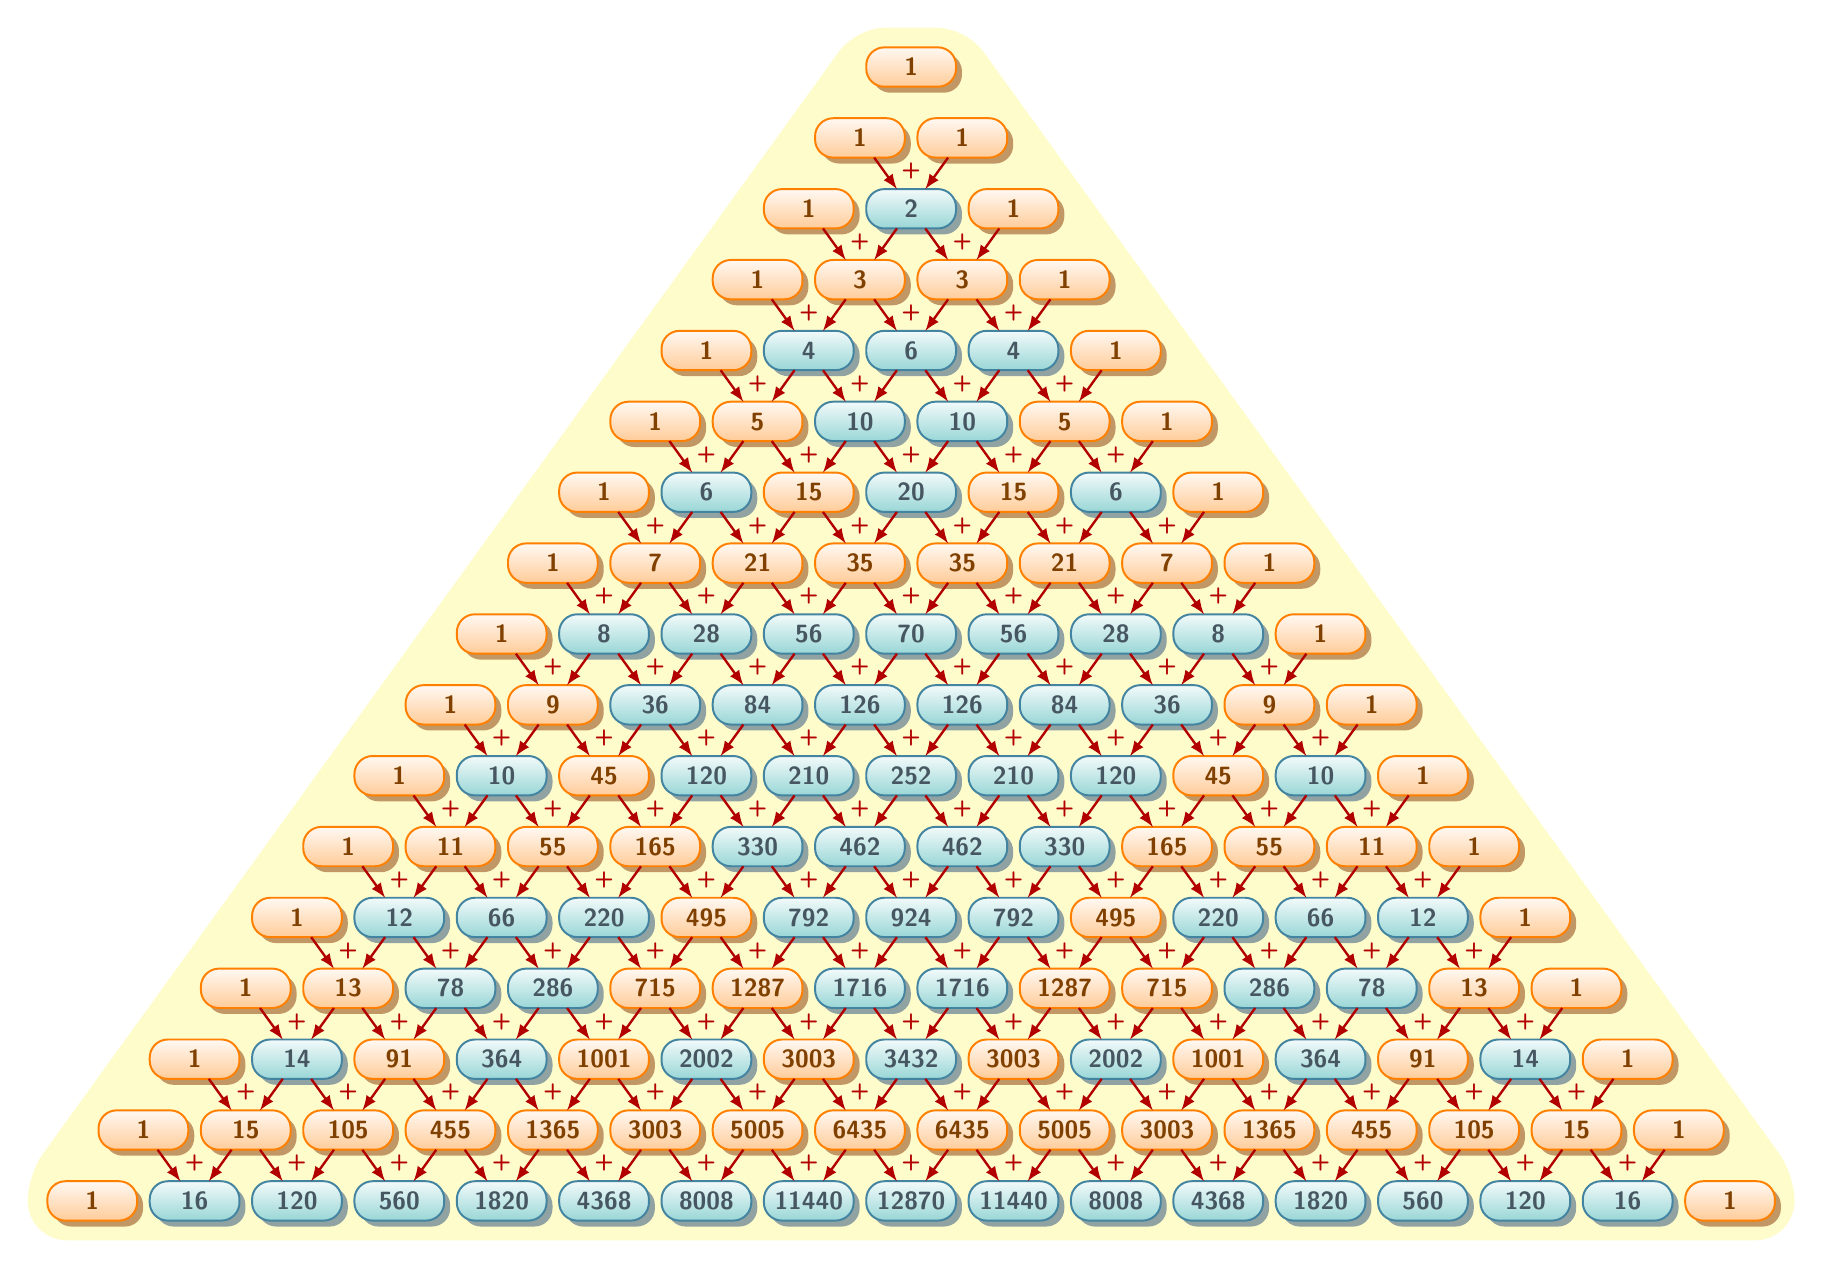
\begin{tikzpicture}[x=13mm,y=9mm]
  % some colors
  \colorlet{even}{cyan!60!black}
  \colorlet{odd}{orange!100!black}
  \colorlet{links}{red!70!black}
  \colorlet{back}{yellow!20!white}
  % some styles
  \tikzset{
    box/.style={
      minimum height=5mm,
      inner sep=.7mm,
      outer sep=0mm,
      text width=10mm,
      text centered,
      font=\small\bfseries\sffamily,
      text=#1!50!black,
      draw=#1,
      line width=.25mm,
      top color=#1!5,
      bottom color=#1!40,
      shading angle=0,
      rounded corners=2.3mm,
      drop shadow={fill=#1!40!gray,fill opacity=.8},
      rotate=0,
    },
    link/.style={-latex,links,line width=.3mm},
    plus/.style={text=links,font=\footnotesize\bfseries\sffamily},
  }
  % Pascal's triangle
  % row #0 => value is 1
  \node[box=odd] (p-0-0) at (0,0) {1};
  \foreach \row in {1,...,16} {
     % col #0 =&gt; value is 1
    \node[box=odd] (p-\row-0) at (-\row/2,-\row) {1};
    \pgfmathsetmacro{\value}{1};
    \foreach \col in {1,...,\row} {
      % iterative formula : val = precval * (row-col+1)/col
      % (+ 0.5 to bypass rounding errors)
      \pgfmathtruncatemacro{\value}{\value*((\row-\col+1)/\col)+0.5};
      \global\let\value=\value
      % position of each value
      \coordinate (pos) at (-\row/2+\col,-\row);
      % odd color for odd value and even color for even value
      \pgfmathtruncatemacro{\rest}{mod(\value,2)}
      \ifnum \rest=0
        \node[box=even] (p-\row-\col) at (pos) {\value};
      \else
        \node[box=odd] (p-\row-\col) at (pos) {\value};
      \fi
      % for arrows and plus sign
      \ifnum \col<\row
        \node[plus,above=0mm of p-\row-\col]{+};
        \pgfmathtruncatemacro{\prow}{\row-1}
        \pgfmathtruncatemacro{\pcol}{\col-1}
        \draw[link] (p-\prow-\pcol) -- (p-\row-\col);
        \draw[link] ( p-\prow-\col) -- (p-\row-\col);
      \fi
    }
  }
  \begin{pgfonlayer}{background}
    % filling and drawing with the same color to enlarge background
    \path[draw=back,fill=back,line width=5mm,rounded corners=2.5mm]
    (  p-0-0.north west) -- (  p-0-0.north east) --
    (p-16-16.north east) -- (p-16-16.south east) --
    ( p-16-0.south west) -- ( p-16-0.north west) --
    cycle;
  \end{pgfonlayer}
\end{tikzpicture}

\end{document}
